\documentclass[10pt,pdf,hyperref={unicode}]{beamer}
\usetheme{Berlin}
\usepackage{graphicx}

\usepackage[utf8]{inputenc}
\usepackage[T1,T2A]{fontenc}
\usepackage{microtype}
\usepackage{amsmath}
\beamertemplatenavigationsymbolsempty

\usepackage[russian, english]{babel}
%----TITLE INFO BEGIN-----
\title[Исследование сечений тессеракта трехмерной гиперплоскостью с использованием методов компьютерного моделирования] % ( long titles)
{ \bfseries Исследование сечений тессеракта гиперплоскостью}
\subtitle{используя методы компьютерного моделирования.}

\author[Максимов Г., Нугманов А., Мустафин И.]
{ \bfseries Максимов Григорий, Нугманов Артур, Мустафин Ильгиз}

\institute[]{
	\vspace{0.2cm}
	{\bfseries Научный руководитель - Давлетбаев Марсель Фанилевич} \\
	\vspace{0.2cm}

  { \normalsize МАОУ "Лицей-интернат №2"} \\
  Московского района города Казани
}

\date[2015-03-26] % (optional)
{Конференция имени Лобачевского 2015}
\subject{Математика}
%-----TITLE INFO END-----

\begin{document}
\frame{\titlepage}

\begin{frame}
\frametitle{Тессеракт. Общее определение}

\begin{columns}
	\column{0.5\textwidth}
		\framebox{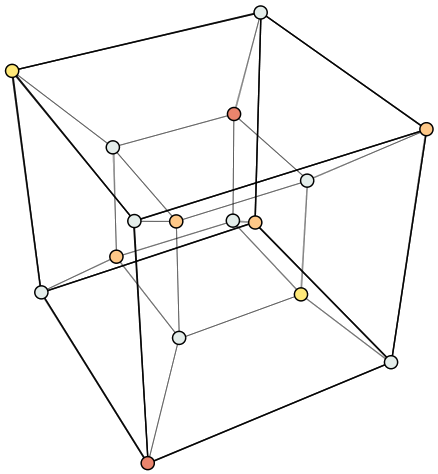
\includegraphics[scale=0.3]{./tesseract_fig1.png}}
	\column{0.5\textwidth}
	{\small
	\begin{itemize}
		\item Рассматриваемая нами модель имеет координаты $(x_1,x_2,x_3,x_4) \in \mathbb{R}^4$, такие, что $x_i \in [ -1,1 ]$. 
		\item Ограничивается 8 гиперплоскостями	
		\item Имеет 8 трехмерных граней, 24 двумерных, 32 ребра и 16 вершин.
	\end{itemize}
}
	\clearpage
\end{columns}

%\begin{columns}
%		\column{0.5\textwidth}
% 			Содержимое левого столбца
% 		\column{0.5\textwidth}
% 			Содержимое правого столбца
%\end{columns}
\end{frame}
\begin{frame}
\frametitle{Наглядный процесс формирования отображения тессеракта на трехмерную плоскость}
\begin{center}
\framebox{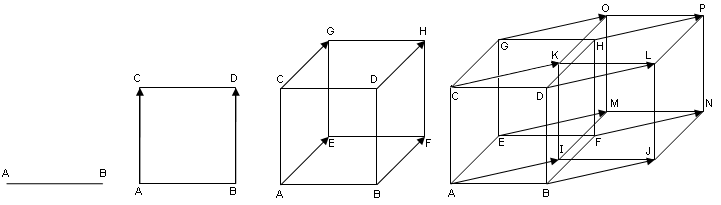
\includegraphics[scale=0.4]{./make_tess.png}}
\end{center} 

Наглядный процесс как точка $A$ переходит постепенно в гиперкуб, приобретая новые размерности
\end{frame}
\begin{frame}
	\frametitle{Лемма о размерности сечений}
%	\setbeamercolor{block title}{use=structure,fg=white,bg=purple!75!black}
%	\setbeamercolor{block body}{use=structure,fg=black,bg=white!20!white}

%	\begin{block}{title 1}
%		...
%	\end{block}
%\setbeamercolor{block title}{use=structure,fg=white,bg=blue!75!black}
{\small
	\begin{block}{Лемма 1}
		Сечением любого $4$-мерного геометрического объекта $3$ мерной гиперплоскостью является геометрическое тело, имеющее размерность не более $3$. 
	\end{block}
}
	\begin{columns}
		\column{0.5\textwidth}
			\framebox{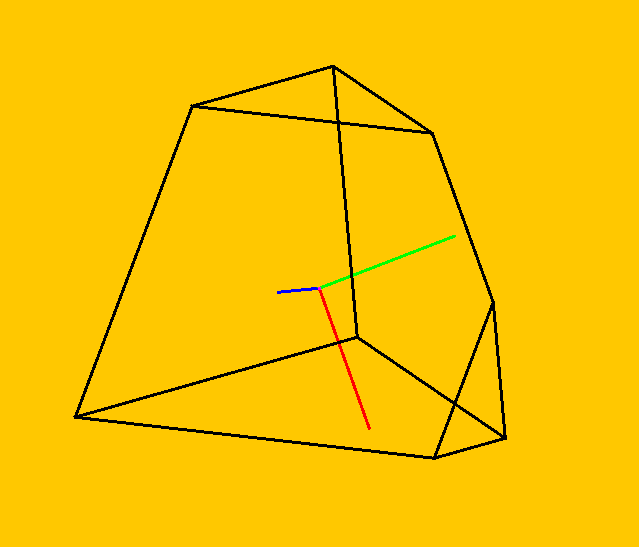
\includegraphics[scale=0.22]{./8.png}}
		\column{0.5\textwidth}
			\framebox{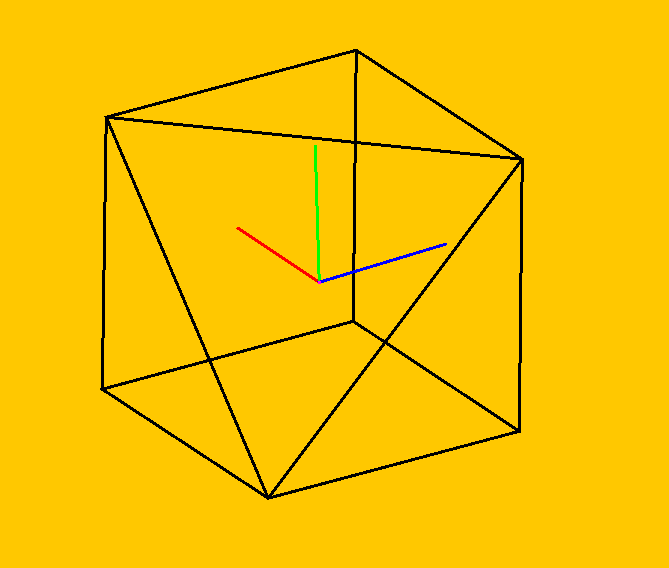
\includegraphics[scale=0.21]{./11.png}}
	\end{columns}
\end{frame}
\begin{frame}
	\frametitle{Лемма о выпуклости}
	\setbeamercolor{block title alerted}{fg=white,bg=black}

	\begin{alertblock}{О выпуклости тессеракта}
		Рассматриваемый в нашей работе тессеракт выпуклый.
	\end{alertblock}

	\begin{block}{Лемма 2}
		Сечением тессеракта гиперплоскостью является выпуклое геометрическое тело.
	\end{block}
\end{frame}
\begin{frame}
	\frametitle{Метод построения сечений тессеракта гиперплоскостью}
	\begin{itemize}
		\item Задание гиперплоскости сечения
		\item Нахождение точек пересечения гиперплоскости и тессеракта
		\item Поворот получившегося сечения до вложимости его в трехмерное пространство
		\item Анализ полученного сечения
	\end{itemize}
	\framebox{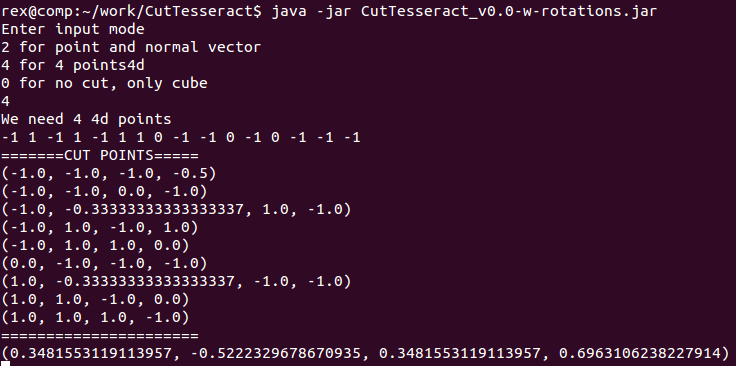
\includegraphics[scale=0.35]{./interface_old.png}}
\end{frame}
\begin{frame}
	\frametitle{Задание гиперплоскости сечения с помощью точек}
	\begin{block}{Гиперплоскость сечения. Уравнение.}
		{\bfseries $ax+by+cz+dw+e=0$} \\ $(a,b,c,d,e)$ - коэффициенты
		

	$		M_1=(x_1,y_1,z_1,w_1) \\
			M_2=(x_2,y_2,z_2,w_2) \\
			M_3=(x_3,y_3,z_3,w_3) \\
			M_4=(x_4,y_4,z_4,w_4)
		$
	\end{block}
	Задается по четырем точкам $(M_1,M_2,M_3,M_4)$ с помощью матрицы: \\

	\begin{flushleft}
	$$ \left|
	\begin{array}{cccc}
		x-x_1 & y-y_1 & z-z_1 & w-w_1     \\
		x_2-x_1 & y_2-y_1 & z_2-z_1 & w_2-w_1    \\
		x_3-x_1 & y_3-y_1 & z_3-z_1 & w_3-w_1      \\
		x_4-x_1 & y_4-y_1 & z_4-z_1 & w_4-w_1 
	\end{array}
	\right|=0
	$$
\end{flushleft}

\end{frame}
\begin{frame}
	\frametitle{Задание гиперплоскости с помощью точки и вектора}
	\begin{block}{}
		Способ во многом аналогичен объявлению обыкновенной двумерной плоскости при помощи нормали к ней и точки, принадлежащей данной плоскости.
	\end{block}
	\begin{block}
		$$
		A(x_1,y_1,z_1,w_1) \mbox{ - произвольная точка} \\
		\overrightarrow N (x_2,y_2,z_2,w_2) \mbox{ - нормаль к искомой гиперплоскости} \\
		P(ax+by+cz+dw+e=0) \\
		\mbox{Свободный член $e$ можно выразить через cледующую формулу} \\
		\newline
		e=-(x_2x_1+y_2y_1+z_2z_1+w_2w_1)
		$$
\end{block}
Таким образом, мы объявили гиперплоскость сечения.
\end{frame}
\begin{frame}
	\frametitle{Нахождение точек пересечения гиперплоскости и тессеракта}
	Пусть $A$ - вершина гиперкуба, $P$ - наша гиперплоскость. \\
	Произведем проверку взаимного расположения вершины тессеракта и гиперплоскости.\\
	\begin{block}{}
	$
		A:=(x_1,y_1,z_1,w_1) \\
		P:=(ax + by + cz + dw + e = 0) \\
		\left[
		\begin{array}{cc}
			ax_1 + by_1 + cz_1 + dw_1 + e = 0 & \mbox{Вершина принадлежит сечению} 
			\\
			ax_1 + by_1 + cz_1 + dw_1 + e > 0 & \mbox{Вершина "выше" плоскости сечения}
			\\
			ax_1 + by_1 + cz_1 + dw_1 + e < 0 & \mbox{Вершина "ниже" плоскости сечения} 
		\end{array}
	$
\end{block} \\

Далее при помощи параметрического уравнения находим точку пересечения.
\end{frame}
\begin{frame}
	\frametitle{Поворот сечения}	\\

	\begin{columns}
		\column{0.5\textwidth}
	\begin{block}{Матрицы поворота в четырехмерном пространстве.}
		{\footnotesize
			$$
			M_{xy}(\alpha)=
			\left(
			\begin{array}{cccc}
				\cos \alpha & -\sin \alpha & 0 & 0 \\
				\sin \alpha & \cos \alpha & 0 & 0 \\
				0 & 0 & 1 & 0 \\
				0 & 0 & 0 & 1
			\end{array}\right)
			$$			\\
			
			\newline
			$$
			M_{yz}(\alpha)=
			\left(
			\begin{array}{cccc}
				1 & 0 & 0 & 0 \\
				0 & \cos \alpha & -\sin \alpha & 0 \\
				0 & \sin \alpha & \cos \alpha & 0 \\
				0 & 0 & 0 & 1
			\end{array}\right)
			$$			\\ 

			$$
			M_{zw}(\alpha)=
			\left(
			\begin{array}{cccc}
				1 & 0 & 0 & 0 \\
				0 & 1 & 0 & 0 \\
				0 & 0 & \cos \alpha & -\sin \alpha \\
				0 & 0 & \sin \alpha & \cos \alpha
			\end{array}\right)
			$$
		}

\end{block}
\column{0.5\textwidth}
\framebox{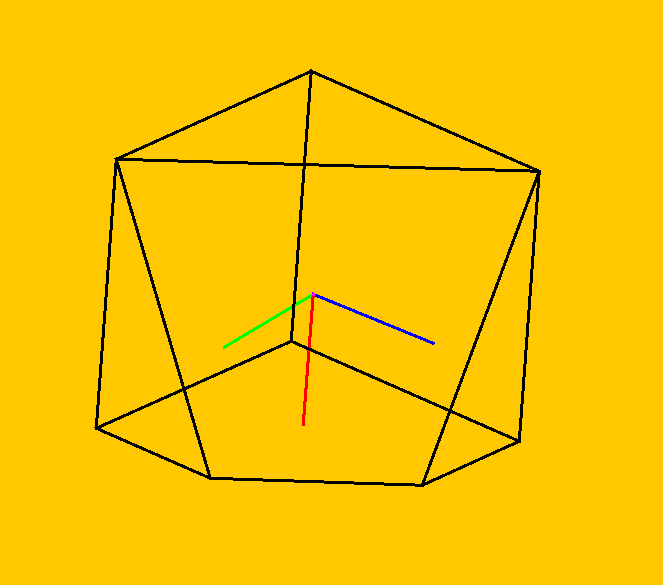
\includegraphics[scale=0.22]{./5.png}}
\end{columns}
\end{frame}

\begin{frame}
	\frametitle{Теорема о параллельности граней противоположных сечений}
	\begin{block}{Теорема 1}
		Грани сечения, полученные пересечением противоположных ячеек тессеракта гиперплоскостью, параллельны.
	\end{block}
\end{frame}
\begin{frame}
	\frametitle{Лемма о четности суммы степеней вершин сечения}
	\begin{block}{Лемма 3}
		Не существует сечений, сумма степеней вершин которых нечетна.
	\end{block}
\end{frame}
\begin{frame}
	\frametitle{Лемма о степени вершин}
	\begin{block}{Лемма 4}
		Трехмерные сечения тессеракта состоят из вершин только со степенями 3 и 4.
	\end{block}
\end{frame}

\begin{frame}
	\frametitle{Теорема о количестве вершин}
	\begin{block}{Теорема 2}
		Трехмерные сечения тессеракта имеют не менее 4 и не более 12 вершин, но не 5.
	\end{block}
	\begin{columns}
		\column{0.5\textwidth}
			\framebox{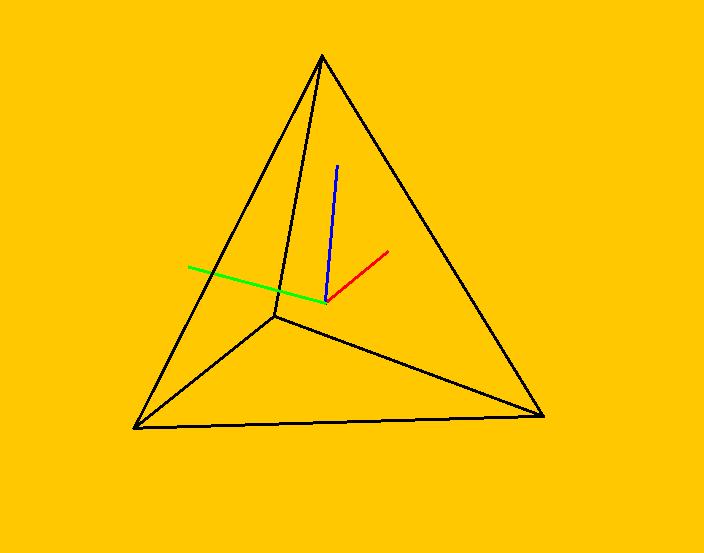
\includegraphics[scale=0.23]{./13.png}}
		\column{0.5\textwidth}
			\framebox{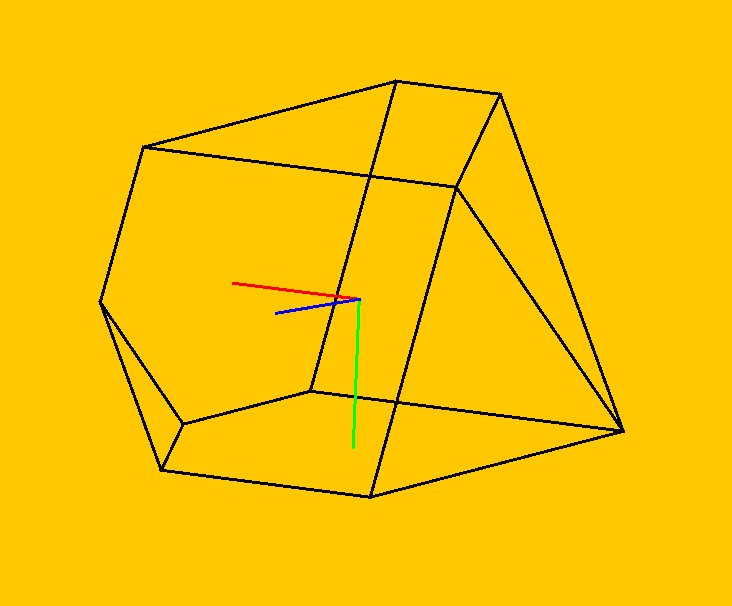
\includegraphics[scale=0.21]{./16.png}}
	\end{columns}
\end{frame}

\begin{frame}
	\frametitle{Заключение}
	\begin{block}{Мы на Github}
		https://github.com/imustafin/CutTesseract
	\end{block}
	\begin{block}{Сайт проекта}
		http://imustafin.github.io/CutTesseract/
	\end{block}
\end{frame}

\begin{frame}
	\vspace{}
\end{frame}
%%%%%%%%%%PROOF%%%%%%%%%%PROOF%%%%%%%%%%%%
%%%%%%%%%%%%%%%%%%%%%%%%%%%%%%%%%%%%%%%%%%
\begin{frame}
	\frametitle{Размерность сечения}
	\begin{block}{Сечение}
		Сечение - это множество точек, принадлежащих, как тессеракту, так и гиперплоскости сечения.
	\end{block}
	Из этого следует вывод о том, что сечение не может иметь размерность более 3, так как размерность секущей гиперплоскости - 3. 
	
\end{frame}
\begin{frame}
	\frametitle{Доказательсто выпуклости сечения}
	\begin{block}{}
		\framebox{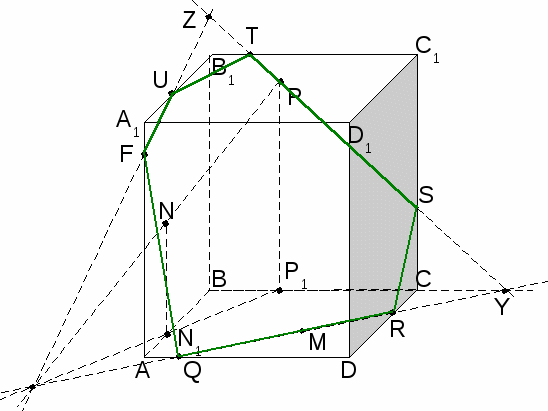
\includegraphics[scale=0.4]{./vipuk.png}}
	\end{block}

		
\end{frame}
\begin{frame}
	\frametitle{Доказательство теоремы 1}
	\begin{equation*}

		P_1 \left\{
		\begin{array}{lc}
			ax+by+cz+dw+e=0 \\
			w=1
		\end{array}\\
		P_2 \left\{
		\begin{array}{lc}
			ax+by+cz+dw+e=0 \\
			w=-1
		\end{array}\\
	a^2+b^2+c^2\ne0
\end{equation*}
	
\end{frame}
\begin{frame}
	\frametitle{Доказательство четности суммы степеней вершин сечения}
	\begin{block}{Лемма о рукопожатиях}
		Любой конечный неориентированный граф имеет чётное число вершин нечётных степеней.
	\end{block}
\end{frame}
\begin{frame}
	\frametitle{Доказательство Леммы о степени вершин}
	Данная лемма является следствием Теоремы 1 о параллельности. \\
	Так как тессеракт состоит из 8 ячеек, пары которых параллельны, то при сечении данного тессеракта гиперплоскостью образуются 4 пары параллельных двумерных плоскостей. \\
	Как следствие, одновременно пересекаться в одной точке могут лишь 4 из них. То есть максимальная степень вершины сечения тессеракта - 4. \\
	Как известно, для получения точки требуется пересечь как минимум три плоскости. Поэтому, минимальная степень вершины сечения - 3.
\end{frame}
\begin{frame}
	\frametitle{Доказательство Теоремы 2 о количестве вершин}
	Как ивестно, для получения трехмерного геометрического тела требуется минимум 4 вершины. \\
	По теореме Эйлера для многогранников: 
	\begin{equation*}
	\left\{
		\begin{array}{lc}
		\mbox{$V$ - количество вершин, $E$ - ребер, $F$ - граней.} \\
		V-E+F=2 \\
		F\le8 \\
		\mbox{Пусть }V=x+y \\
		\mbox{$x$ - количество вершин со степенью 3}\\ 
		\mbox{$y$ - количество вершин со степенью 4} \\
		E=\frac{3x+4y}{2}, 
		\mbox{ по лемме о рукопожатиях и лемме о степени вершин}\\
	\end{array}
\end{equation*}
\end{frame}
\begin{frame}
	\frametitle{Доказательство Теоремы 2 о количестве вершин}
	{\Large
	\begin{equation*}
	\begin{array}{lc}
		\mbox{$V$ - количество вершин, $E$ - ребер, $F$ - граней.} \\
		F=2-E+V \\
		2-V+E\le8 \\
		E-V\le6 \\
	%	\noindent\rule{2cm}{0.4pt} \\
		\mbox{ }\\
		\frac{3x+4y}{2}-x-y\le6\\
		x+2y\le12 \\
		V=x+y\le x+2y\le12\\
	}
	{\normalsize
		\mbox{Таким образом мы нашли верхний предел степени вершины сечения}
	}

	\end{array}
\end{equation*}
	
\end{frame}
\begin{frame}
	\frametitle{Доказательство Теоремы 2 о количестве вершин}
	Рассмотрим все графы с 5 вершинами, имеющие степень 3 и 4.\\
\hfill \break	
	{\large	
		33333 - не может быть по Лемме о четности\\
		33334 - может быть\\
		33344 - не может быть по Лемме о четности\\
		33444 - может быть\\
		34444 - не может быть по Лемме о четности\\
		44444 - не планарный граф
\\	
\hfill \break	
	Таким образом остаются два графа, потенциально нам подходящие.
}
\end{frame}
\begin{frame}
	\frametitle{Доказательство Теоремы 2 о количестве вершин}
	\begin{columns}
		\column{0.5\textwidth}
		{\large $33334$}
		\framebox{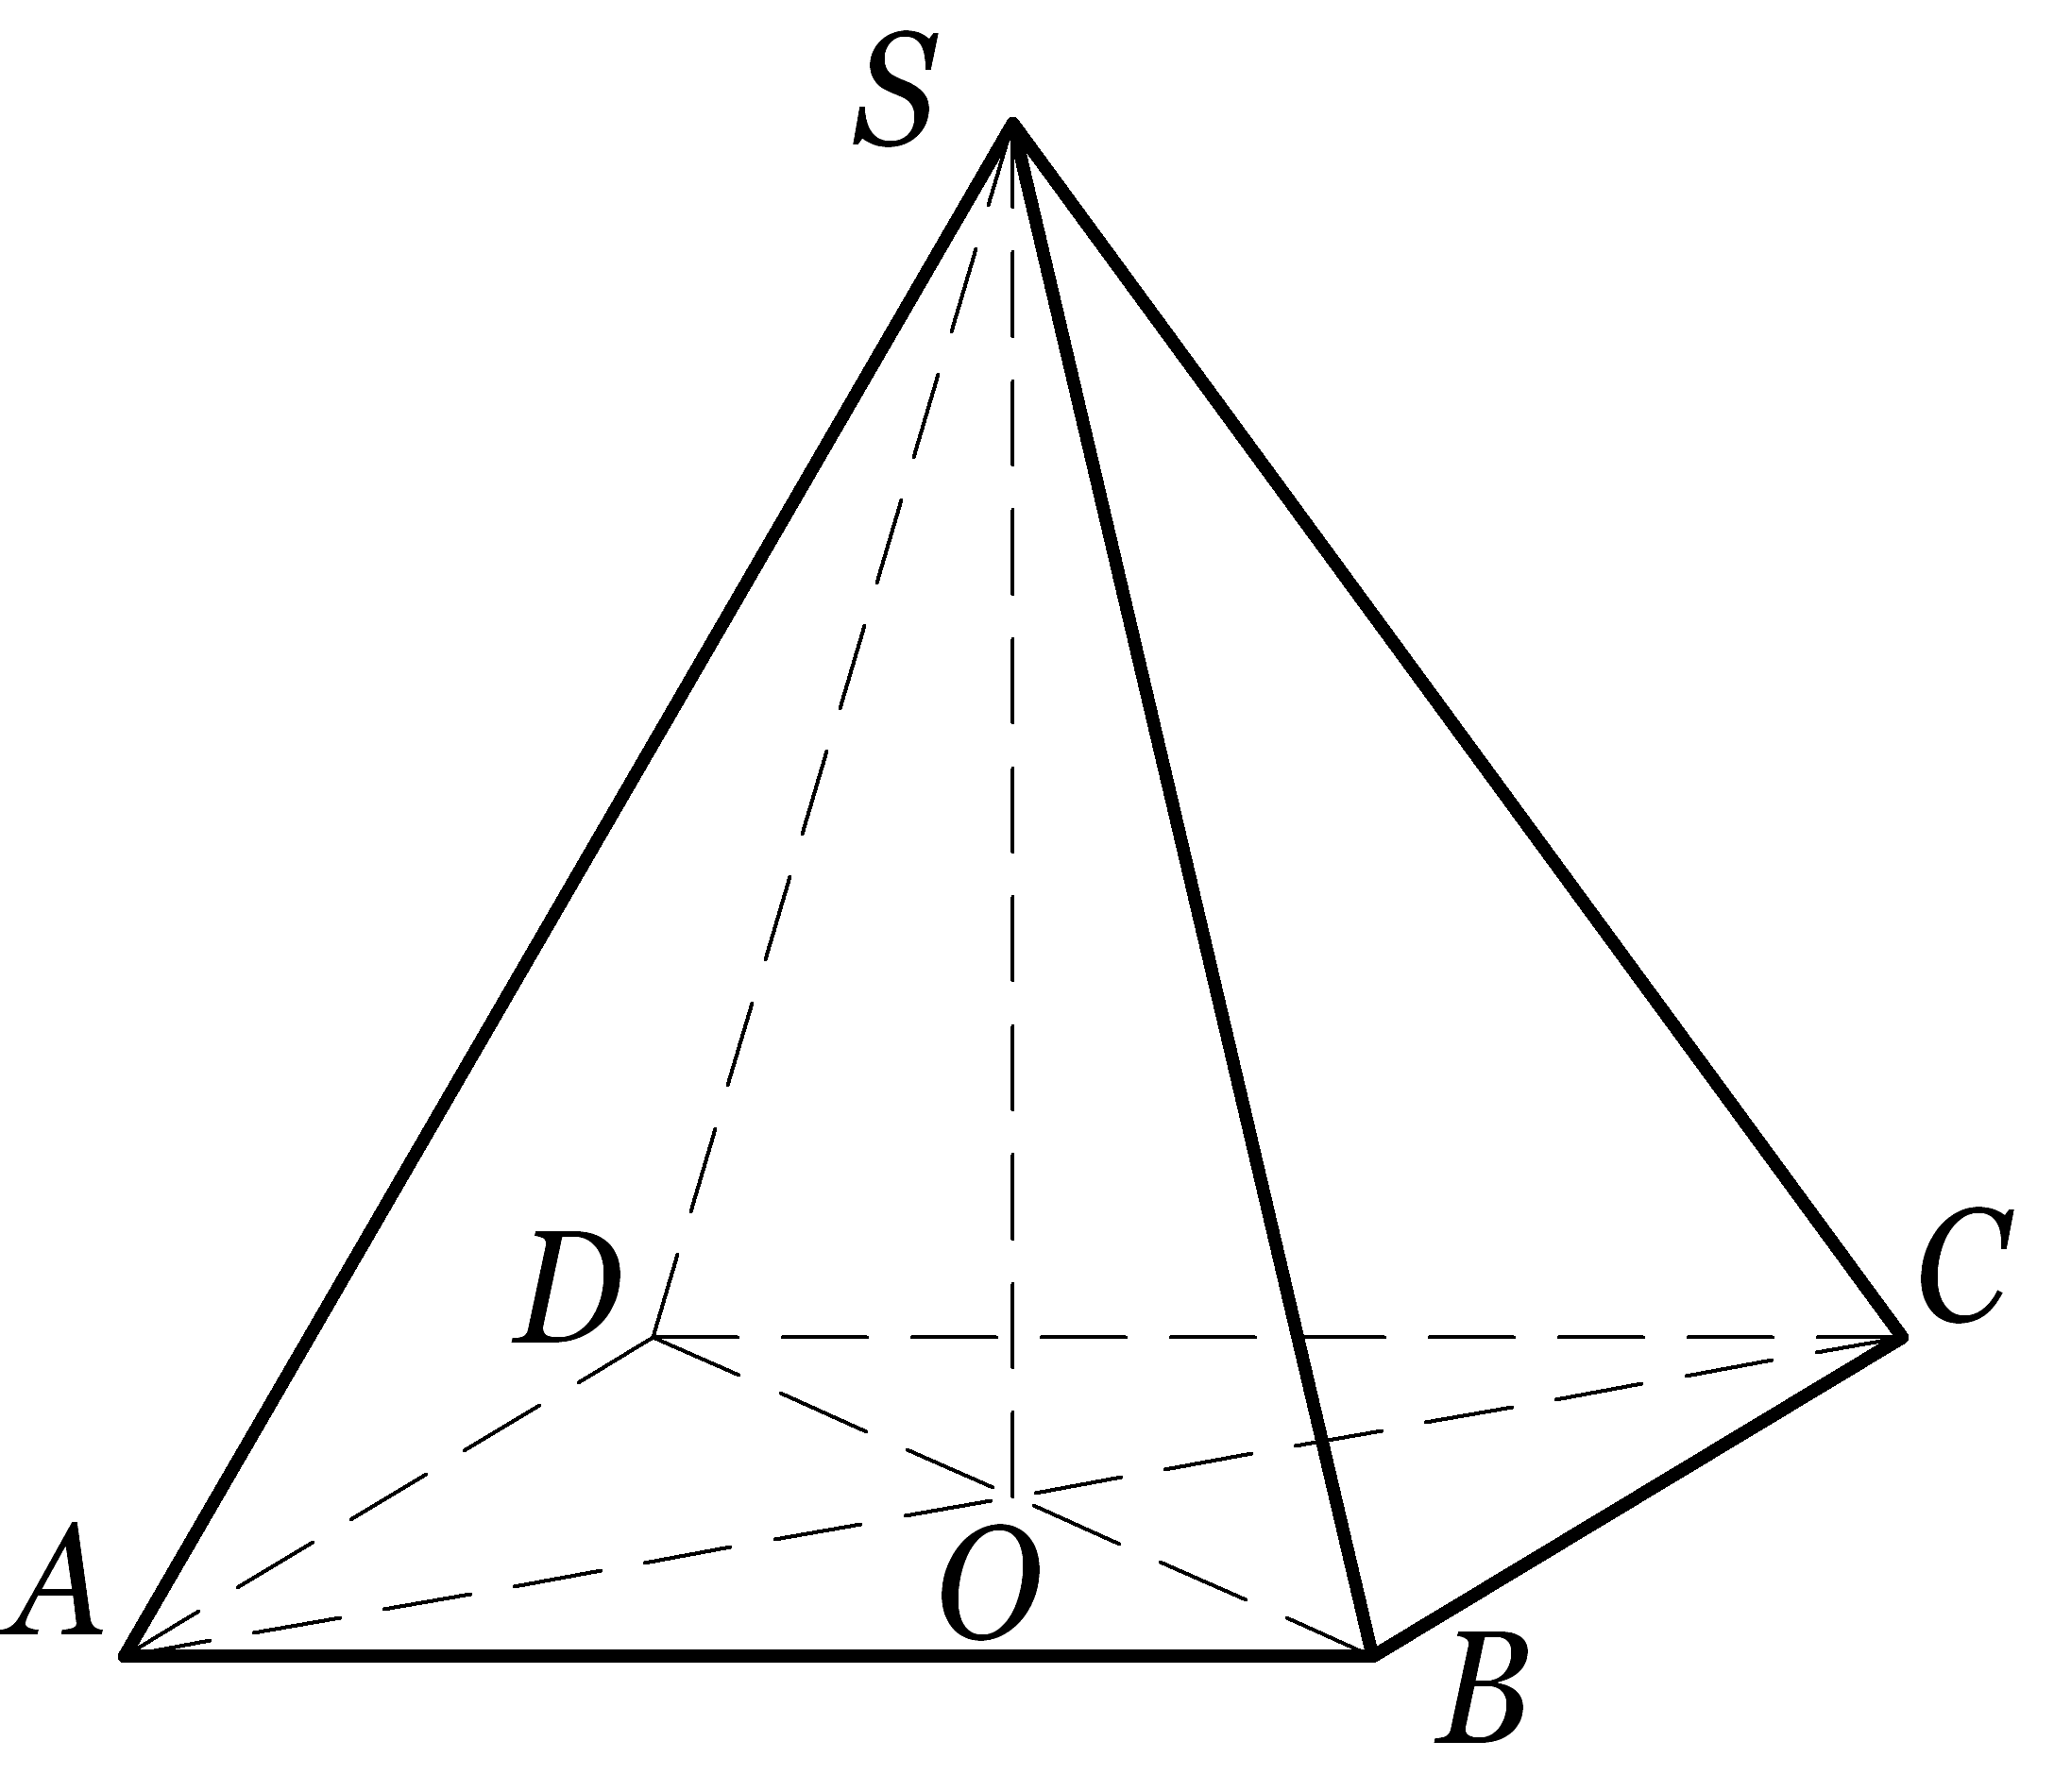
\includegraphics[scale=0.1]{./4pyramid}}

		\column{0.5\textwidth}
		{\large $33444$}
		\framebox{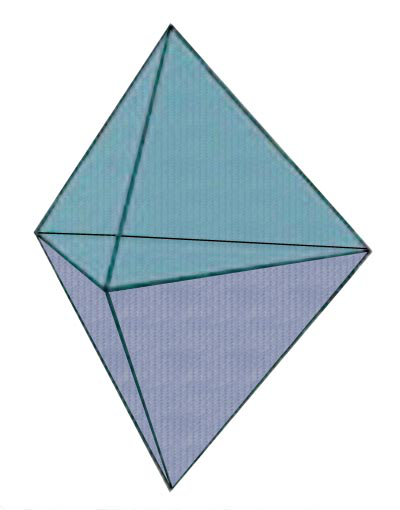
\includegraphics[scale=1.94]{./bipyramid.png}}
	\end{columns}
	Они не являются сечениями гиперкуба, так как у них более 4 граней и нет ни одной пары параллельных.
\end{frame}
\end{document}

